\newpage
\subsubsection{ALS XY Wing}
Bei der Technik \textit{ALS XY Wing} benötigt man 3 \textit{ALS} A, B und C. A und C haben den gemeinsamen \textit{RCC} X, B und C haben den gemeinsamen \textit{RCC} Y. X und Y sind unterschiedlich. \textit{ALS} A und B haben die gemeinsame Ziffer Z, die kein \textit{RCC} ist.\\
Nun werden zwei Fälle betrachtet. Wenn Z nicht in A steht, dann muss X in A stehen, da bei einem \textit{ALS} nur eine Ziffer fehlen darf. Das bedeutet, C muss Y enthalten, da Z nicht in C steht. Daraus kann man folgern, dass B den Kandidaten Z enthalten muss. Im Fall zwei nehmen wir an, dass Z nicht in B steht. Dann muss Y in B stehen, woraus folgt, dass X in B steht. Daher muss dann Z in A stehen. In jedem möglichen Fall steht Z also entweder in A oder in B. Daher können alle Kandidaten von Z ausgeschlossen werden, die von allen Instanzen in A und B gesehen werden.

\begin{figure}[h]
\begin{center}
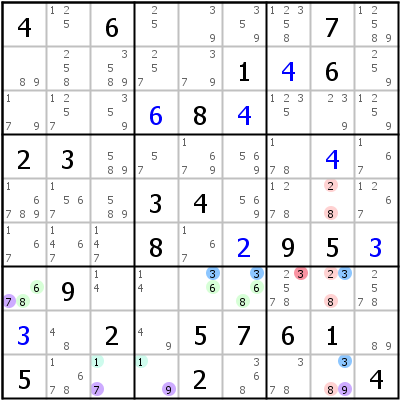
\includegraphics{./img/ALS_XY_Wing.png}
\caption{ALS XY Wing}
\end{center}
\end{figure}

Im oben stehenden Beispiel \textbf{Abbildung 4.19} sieht man einen \textit{ALS XY Wing}, \textit{ALS} A ist hier Zeile 7 Spalten 1, 5 und 6 mit den Kandidaten 3, 6, 7 und 8, B ist Spalte 8 Zeilen 5, 7 und 9 mit den Kandidaten 2, 3, 8 und 9. \textit{ALS} C befindet sich in Zeile 9 Spalten 3 und 4 mit den Kandidaten 1, 7 und 9. X ist also 7, Y ist 9 und Z ist 3. Da Z wegen der oben genannten Begründung nur in \textit{ALS} A und B vorkommen kann, können jetzt alle Kandidaten von Z gelöscht werden, die von allen Instanzen von Z in A und B gesehen werden. Das ist die Ziffer 3 in z7s7.